\section{Multi-domain system modeling (1 page)}
\label{section:contribution_1}

Our approach is based on emergent property estimation techniques \cite{hackenberg2012towards} and uses a model-based approach for validating requirements in early phases of development proposed in \cite{hackenberg2014rapid}, relying on partial system models to ease modeling effort. An adaption to the ITS domain of this modeling technique was proposed in \cite{ascher2014early}, facilitating the formulation of multi-objective traffic flows as an optimal control problem consisting of state variables, control variables, constraints and objectives. The approach employs a generic solver for system behavior estimation, which utilizes stochastic optimization techniques.

\begin{figure}[h]
	\centering
	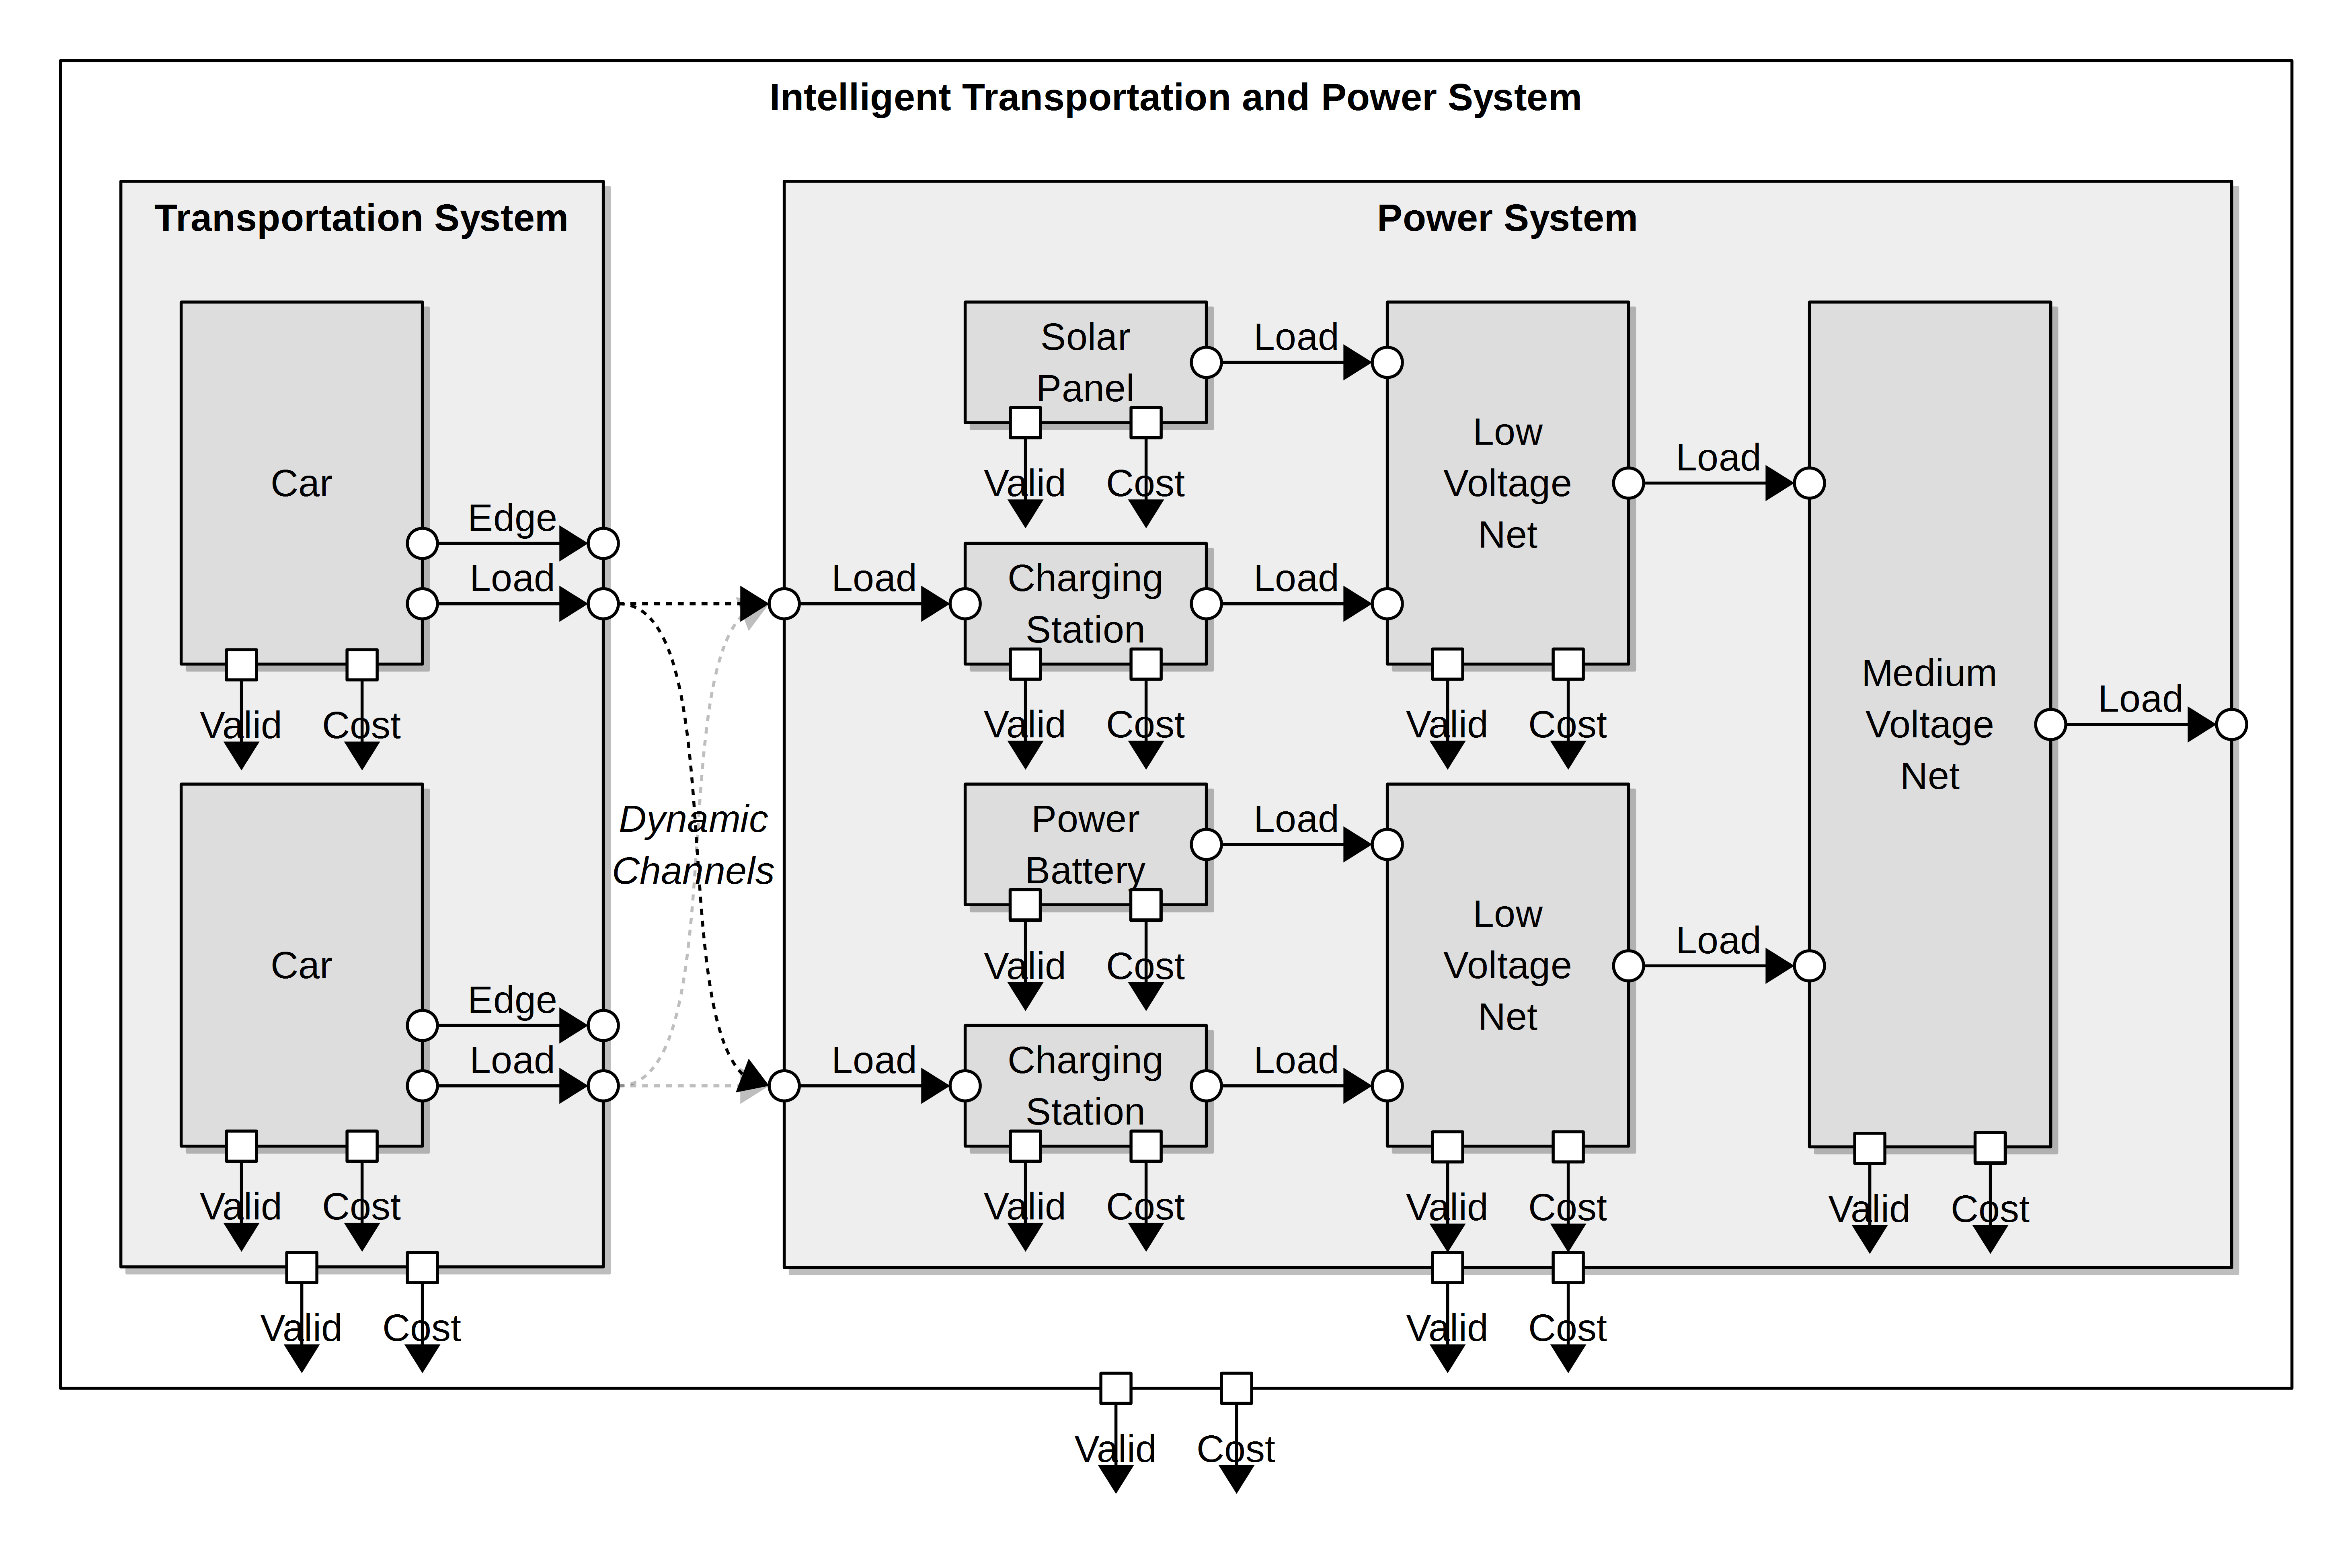
\includegraphics[width=\columnwidth]{../gfx/model.png}
	\caption{Overview of the multi-domain system modeling approach including the transportation system and the electricity network.}
	\label{fig:model}
\end{figure}

Subsequently we describe the different components of the model architecture based on their state variables, control variables, constraints and objectives. 

\subsection{Transportation System}

TBD

\subsection{Electric Network}

TBD

\subsection{Integrated System}

TBD